\documentclass[12pt]{article}


% -------------------- PAQUETES --------------------
\usepackage[utf8]{inputenc}
\usepackage[spanish]{babel}
\usepackage[margin=2.54cm]{geometry}
\usepackage{graphicx}
\usepackage{xcolor}
\usepackage{enumitem}
\usepackage{parskip}
\usepackage{hyperref}
\usepackage{ulem} 
\usepackage{subcaption}


% -------------------- CARGA DE ARCHIVOS EXTERNOS --------------------
% ----------------- UTILIDADES PARA DAR UN MEJOR FORMATO DE DOCUMENTO -----------------  


\definecolor{azul}{rgb}{0.0039, 0.3098, 0.6196}


% Formato para el indice general ...........
\makeatletter
    \renewcommand{\@dotsep}{1.5}
    \renewcommand{\l@section}{\@dottedtocline{1}{1.5em}{2.3em}}
    \renewcommand{\l@subsection}{\@dottedtocline{2}{3.8em}{3.2em}}
    \renewcommand{\l@subsubsection}{\@dottedtocline{3}{7.0em}{4.1em}}
\makeatother

% --------- COMANDOS PERSONALIZADOS PARA LA PORTADA DE LAS TAREAS, TRABAJOS Y PROYECTOS ---------

\newcommand{\rutaLogo}[1]{\newcommand{\RutaLogo}{#1}}
\newcommand{\tema}[1]{\newcommand{\Tema}{#1}}
\newcommand{\etiquetaAutores}[1]{\newcommand{\EtiquetaAutores}{#1}}
\newcommand{\alumno}[1]{\newcommand{\Alumno}{#1}}
\newcommand{\materia}[1]{\newcommand{\Materia}{#1}}
\newcommand{\docente}[1]{\newcommand{\Docente}{#1}}
\newcommand{\ciclo}[1]{\newcommand{\Ciclo}{#1}}
\newcommand{\fecha}[1]{\newcommand{\Fecha}{#1}}
\newcommand{\periodo}[1]{\newcommand{\Periodo}{#1}}



% -------------------- DEFINICIÓN DE LA PORTADA --------------------
\rutaLogo{../../../../gdocs/img/logo-ista.png}
\tema{\\ \vspace{0.5cm} Guía Practica N°3 - Kaggle, OpenRefine y Weka como herramientas para el análisis de datos \\ \vspace{1.2cm}}
\etiquetaAutores{Integrantes:}
\alumno{Eduardo Mendieta\\Freddy Montalván\vspace{0.7cm}}
\materia{Introducción a Big Data \vspace{0.7cm}}
\docente{MSc. Ing. Carmen Tacuri Vintimilla \vspace{0.7cm}}
\ciclo{Primer Ciclo \vspace{0.7cm}}
\fecha{22 de julio de 2024 \vspace{0.7cm}}
\periodo{Abril 2024 - Agosto 2024}


\begin{document}

    \begin{titlepage}

    \centering

    \includegraphics[width=0.11\textwidth]{\RutaLogo} 

    \vspace{0.3cm}
    \textcolor{azul}{\Large \textbf{Instituto Superior Universitario Tecnológico del Azuay \\}}
    \vspace{0.3cm}
    \textcolor{azul}{\Large \textbf{Tecnología Superior en Big Data}}
    
    % 1. ---------------- TEMA -------------------------
    
    {\Large\textbf{\Tema}}
    
    % 2. ---------------- AUTOR(ES) -------------------------
    \textcolor{azul}{\large \textbf{\EtiquetaAutores} \\}
    \vspace{0.3cm}
    {\large \Alumno}

    % 3. ---------------- MATERIA -------------------------
    \textcolor{azul}{\large \textbf{Materia:} \\}
    \vspace{0.3cm}
    {\large \Materia}


    % 3. ---------------- DOCENTE -------------------------
    \textcolor{azul}{\large \textbf{Docente:} \\}
    \vspace{0.3cm}
    {\large \Docente}


    % 3. ---------------- Ciclo -------------------------
    \textcolor{azul}{\large \textbf{Ciclo:} \\}
    \vspace{0.3cm}
    {\large \Ciclo}


    % 3. ---------------- FECHA -------------------------
    \textcolor{azul}{\large \textbf{Fecha:} \\}
    \vspace{0.3cm}
    {\large \Fecha}

    % 3. ---------------- PERIODO -------------------------
    \textcolor{azul}{\large \textbf{Periodo Académico:} \\}
    \vspace{0.3cm}
    {\large \Periodo}
 
\end{titlepage}


    \tableofcontents
    \newpage

    \section*{\centering Guía Practica N°3: Kaggle, OpenRefine y Weka como herramientas para el análisis de datos}

    % 1.Introducción: ...................................................
    \section{Introducción}
        La capacidad de analizar datos de manera efectiva se ha convertido en una habilidad fundamental en el panorama actual, donde la información abunda y su interpretación correcta puede proporcionar insights valiosos para la toma de decisiones informadas. Dentro de este contexto, herramientas como Kaggle, OpenRefine y Weka se destacan como recursos indispensables para aprender y aplicar técnicas de análisis de datos de manera práctica y accesible.
        
        Kaggle destaca como una plataforma central para aprender análisis de datos, ofreciendo conjuntos de datos reales y desafíos competitivos que permiten aplicar técnicas avanzadas de aprendizaje automático. OpenRefine simplifica la limpieza y preparación de datos con una interfaz intuitiva, ideal para principiantes en análisis de datos. Weka ofrece una amplia gama de algoritmos de aprendizaje automático y una interfaz gráfica intuitiva, facilitando la experimentación con técnicas como clasificación, regresión y agrupamiento.
        
        Utilizando un dataset real como el del naufragio del Titanic, estas herramientas se vuelven especialmente relevantes al aplicarlas directamente en un contexto práctico. Este dataset histórico no solo proporciona datos reales para el análisis, sino que también motiva el aprendizaje al enfrentar problemas reales de ciencia de datos. Así, los estudiantes puedemos desarrollar habilidades fundamentales mientras exploramos las capacidades de Kaggle, OpenRefine y Weka en la manipulación y análisis de datos significativos.

    % 2.Objetivos: ...................................................
    \section{Objetivos}
        \subsection{Objetivo general}
            Abordar los ejercicios prácticos delineados en la guía para fomentar el pensamiento analítico a través de la aplicación de herramientas especializadas como Kaggle, OpenRefine y Weka.

        \subsection{Objetivos específicos}
            \begin{itemize}
                \item Instalar las herramientas OpenRefine y Weka siguiendo los pasos de instalación proporcionados en los enlaces de descarga recomendados.
                \item Descargar el archivo titanic.csv desde la plataforma Kaggle para su análisis posterior.
                \item Utilizar OpenRefine para preparar y limpiar los datos del archivo titanic.csv, siguiendo los procedimientos descritos en la guía práctica.
                \item Realizar un análisis gráfico de los datos previamente limpiados con OpenRefine utilizando Weka, siguiendo los procedimientos descritos en la guía práctica.
                \item Presentar los resultados del análisis previo de los datos.
            \end{itemize}

    % 3.Paso a Paso: ...................................................
    \section{Paso a paso}
            \subsection{Kaggle Datasets}
                \href{https://www.kaggle.com/datasets}{\uline{Kaggle Datasets}} es una plataforma en línea que forma parte de la comunidad de Kaggle, ofreciendo una amplia variedad de conjuntos de datos para proyectos de ciencia de datos, análisis y aprendizaje automático. Los usuarios pueden buscar, explorar y descargar datasets en diversos formatos y temáticas, desde datos de salud hasta imágenes y textos. La plataforma facilita la colaboración a través de Notebooks de Kaggle, donde los usuarios pueden analizar datos, construir modelos y compartir sus resultados. Además, los datasets a menudo están asociados con competiciones y proyectos, y la comunidad activa permite discutir y aprender de otros científicos de datos.

            \subsection{OpenRefine}
                OpenRefine es una poderosa herramienta gratuita y de código abierto para trabajar con datos desordenados: limpiarlos, transformarlos de un formato a otro, y extenderlos con servicios web y datos externos.
                
                \begin{itemize}
                    \item En primer lugar, es necesario contar con una versión de Java igual o superior a \textit{Java 8}. Para ello, descargamos la versión adecuada para Ubuntu desde su repositorio oficial utilizando los siguientes comandos: \textit{sudo apt update}, \textit{sudo apt install openjdk-17-jdk} y \textit{java --version}.
                        \begin{figure}[!h]
                            \centering
                            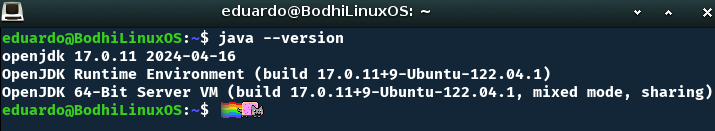
\includegraphics[width=0.8\textwidth]{img/openrefine-1.png}
                            \caption{Verificación de la instalación de Java}
                        \end{figure}
            
                    \item Descargamos \href{https://openrefine.org/download}{\uline{OpenRefine}} desde su página oficial, seleccionando la versión para el sistema operativo Ubuntu. Esto descargará un archivo \textit{.tar.gz}, el cual descomprimimos en el directorio \textit{/home}. A continuación, ingresamos en la carpeta descomprimida y otorgamos permisos de ejecución al archivo refine utilizando el comando \textit{chmod +x refine}. Posteriormente, ejecutamos el archivo con \textit{./refine}. Este proceso iniciará un servidor que se abrirá automáticamente en un navegador, permitiéndonos comenzar a utilizar la herramienta.
                        \newpage
                        \begin{figure}[!h]
                            \centering
                            \begin{subfigure}[b]{0.7\textwidth}
                      
                                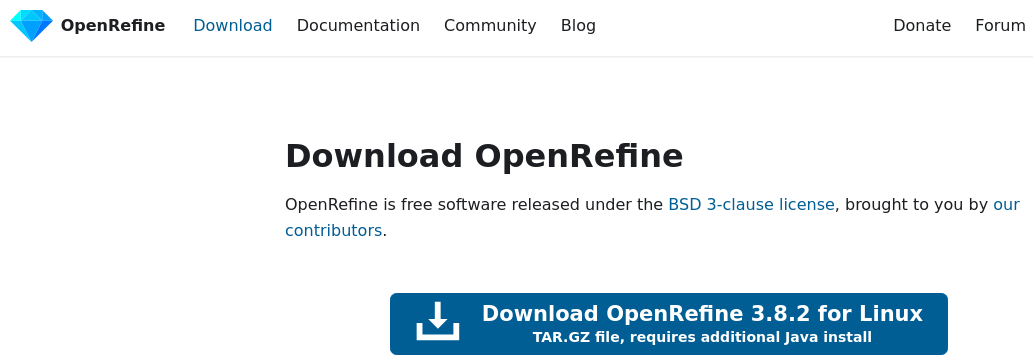
\includegraphics[width=\textwidth]{img/openrefine-2.png}
                            \end{subfigure}
                            \hfill
                            \begin{subfigure}[b]{0.4\textwidth}
                               
                                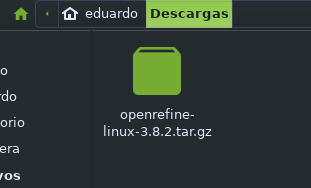
\includegraphics[width=\textwidth]{img/openrefine-3.png}
                            \end{subfigure}
                            \hfill
                            \begin{subfigure}[b]{0.7\textwidth}
                                
                                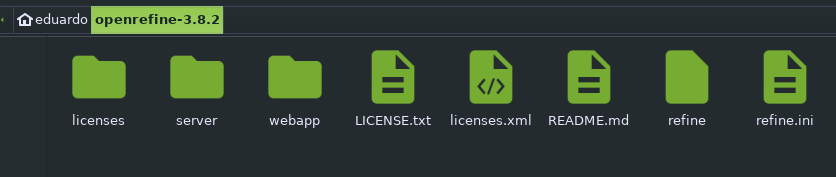
\includegraphics[width=\textwidth]{img/openrefine-4.png}
                            \end{subfigure}
                            \hfill
                            \begin{subfigure}[b]{0.7\textwidth}
                                
                                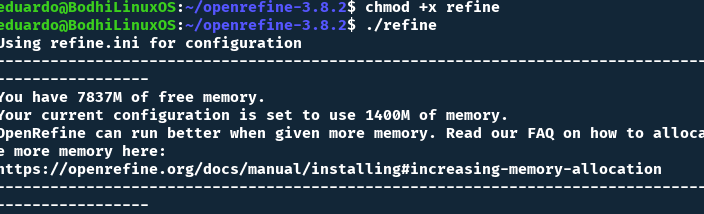
\includegraphics[width=\textwidth]{img/openrefine-5.png}
                            \end{subfigure}
                            \hfill
                            \begin{subfigure}[b]{0.6\textwidth}
                                
                                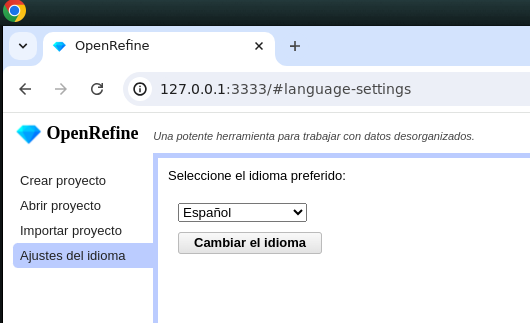
\includegraphics[width=\textwidth]{img/openrefine-6.png}
                            \end{subfigure}
                            \caption{Intalación y ejecución de OpenRefine}
                        \end{figure}
                    
                    \item Procedemos a descargar el archivo \textit{titanic.csv} desde la plataforma \textit{Kaggle} o desde la direccion de \href{https://drive.google.com/file/d/18GdoN1tn_qFFuMn014JFniuoTv4uxrh-/view}{\uline{Google Drive}} propuesta en la guía.
                    \item Podemos cambiar el idioma desde la opción de \textit{Language Settings} del menu latel izquierdo de la herramienta a español.
                    \item Creamos un nuevo proyecto y cargamos el archivo \textit{titanic.csv} previamente descargado, dando clic en \textit{siguiente} y en \textit{Crear Proyecto} en la esquina superior derecha.
                        \begin{figure}[!h]
                            \centering
                            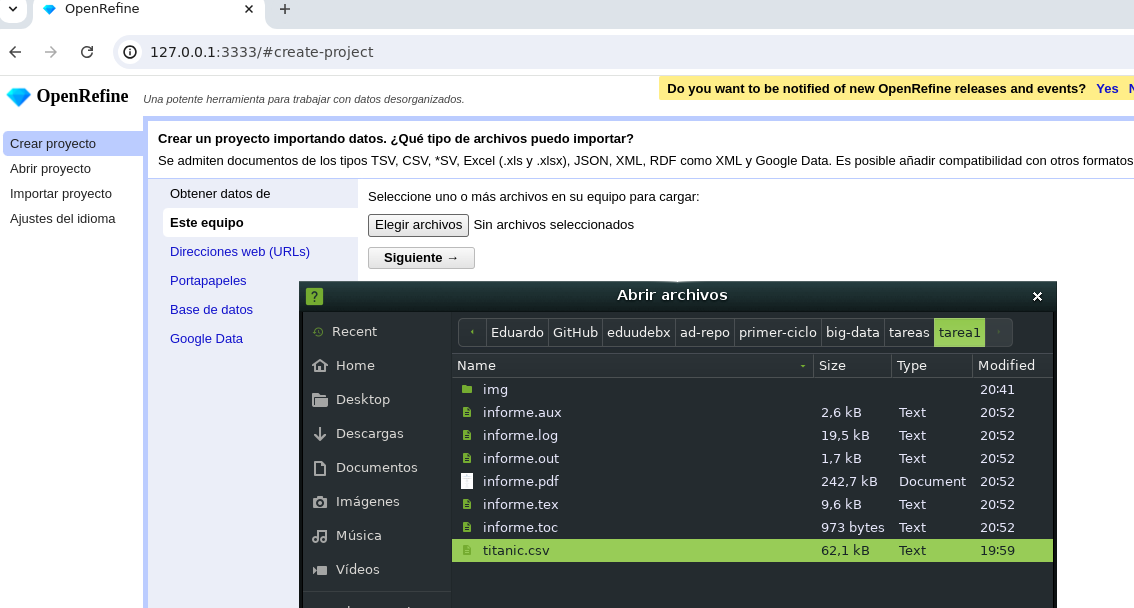
\includegraphics[width=0.9\textwidth]{img/openrefine-7.png}
                            \caption{Creación de un nuevo proyecto}
                        \end{figure}
                    
                    \item Podemos renombrar las columnas, en el caso de la columna \textit{Column}, la podemos renombra a \textit{Vacia}.
                        \begin{figure}[!h]
                            \centering
                            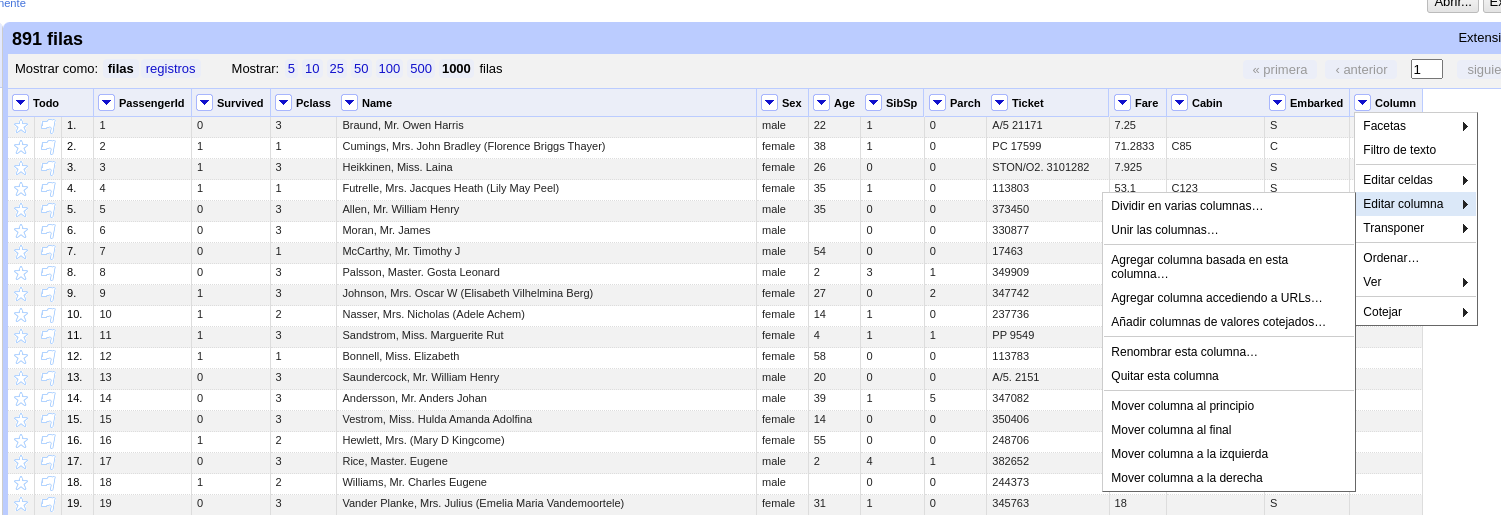
\includegraphics[width=1\textwidth]{img/openrefine-8.png}
                            \caption{Renombrando columnas}
                        \end{figure}
                   
                    \newpage
                    \item En el siguiente paso buscamos los valores no vacios por columna en todo el proyecto dando clic en la columna \textit{Todo $\rightarrow$ Facetas $\rightarrow$ Valores no vacíos por columna}.
                        \begin{figure}[!h]
                            \centering
                            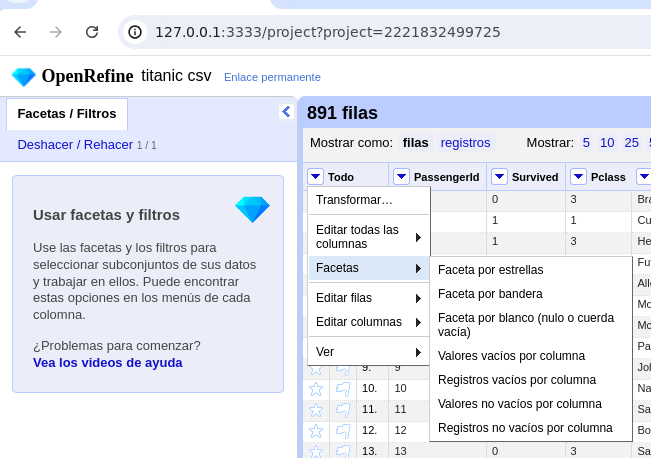
\includegraphics[width=0.7\textwidth]{img/openrefine-9.png}
                            \caption{Buscando valores no vacios por columna}
                        \end{figure}
                    
                    \item Se puede observar que el número total de registros por columna es diferente, por lo cuál podemos inferir que existen valores que no estan definidos dentro de estas, por lo que será necesario tratarlos.
                        \begin{figure}[!h]
                            \centering
                            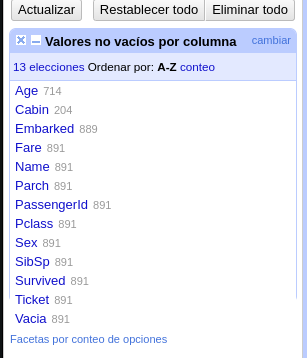
\includegraphics[width=0.4\textwidth]{img/openrefine-10.png}
                            \caption{Valores no vacios por columna}
                        \end{figure}
                    
                    \item Procedemos a retirar la columna \textit{Vacia} puesto que ya no es de utilidad.
                        \begin{figure}[!h]
                            \centering
                            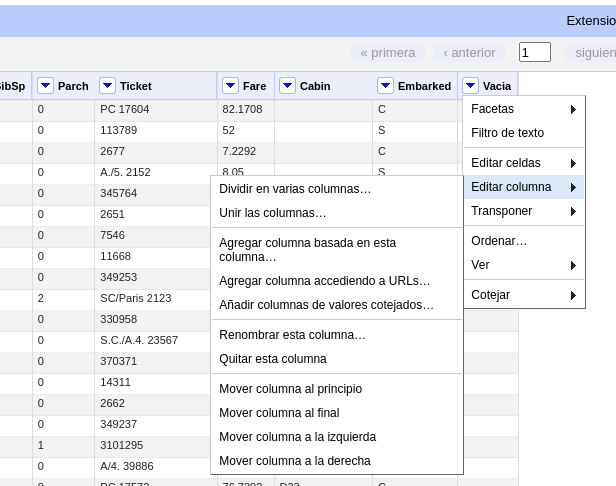
\includegraphics[width=0.4\textwidth]{img/openrefine-11.png}
                            \caption{Eliminando columna \textit{Vacia}}
                        \end{figure}
                    
                    \item La información cargada inicialmente en el proyecto esta en formato de cadena por lo que seria conveniente transformar las columnas que contienen valores numericos, siendo estas \textit{Survived, PClass, Sibsp y Parch} como números enteros y \textit{Age y Fare} en formato decimal.
                        \begin{figure}[!h]
                            \centering
                            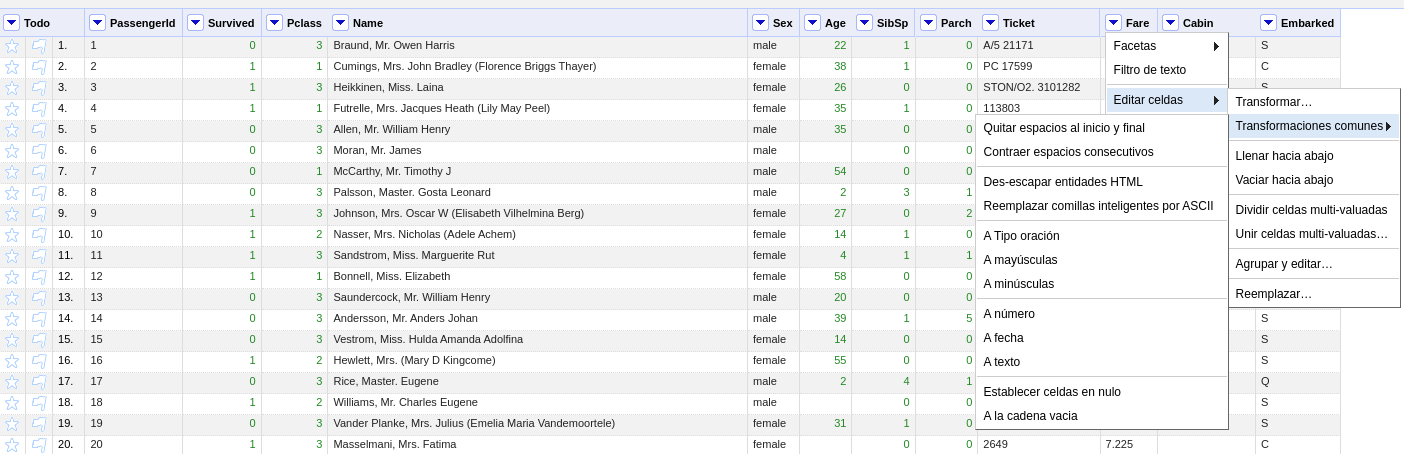
\includegraphics[width=1\textwidth]{img/openrefine-12.png}
                            \caption{Transformación de columnas a tipo numerico}
                        \end{figure}

                    \item Podemos observar los valores vacios por columna en todo el proyecto dando clic en la columna \textit{Todo $\rightarrow$ Facetas $\rightarrow$ Valores vacíos por columna}. Podemos observar que las columnas \textit{Age, Cabin} y \textit{Embarked} contienen valores nulos, por lo que debemos tratar estas columnas.
                        \newpage
                        \begin{figure}[!h]
                            \centering
                            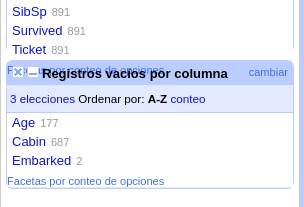
\includegraphics[width=0.4\textwidth]{img/openrefine-13.png}
                            \caption{Columnas con valores nulos}
                        \end{figure}
                    
                    \item Entonces, para completar los valores que faltan en el atributo Embarked, solo lo llenamos con \textit{S} sabiendo que los pasajeros realmente embarcaron en Southampton. Para lo cual filtramos por el valor faltante, al dar click en el panel de resumen en el atribtuto \textit{Embarked}, luego, en la columna \textit{Embarked $\rightarrow$ Editar celdas $\rightarrow$ Reemplazar $\rightarrow$ Reemplazar por} actulizando de esta manera las casillas vacías por la letra \textit{S}.
                        \begin{figure}[!h]
                            \centering
                            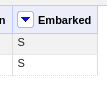
\includegraphics[width=0.3\textwidth]{img/openrefine-14.png}
                            \caption{Reemplazando valores nulos}
                        \end{figure}
                    
                    \item Para el atributo \textit{Cabin}, al no saber la cabina real de cada pasajero, podemos agregar una columna adicional basada en esta llamada \textit{HaveCabin} con un \textit{1} pasajero si la cabina existe y \textit{0} si no existe. Esto se puede lograr con \textit{Cabin $\rightarrow$ Editar columna $\rightarrow$ Agregar columna basada en esta columna}. Agregamos el nombre \textit{HaveCabin} y la siguiente linea de código \textit{if(value.toString() == '', 0, 1)}. por último click en \textit{Aceptar}.
                        \newpage
                        \begin{figure}[!h]
                            \centering
                            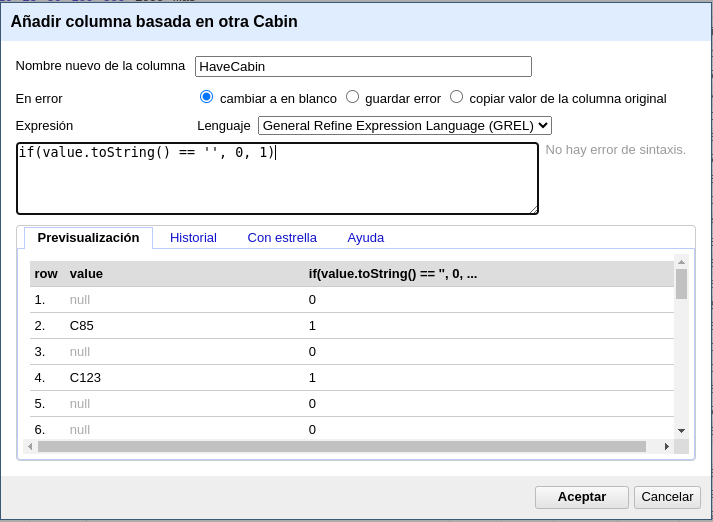
\includegraphics[width=0.6\textwidth]{img/openrefine-15.png}
                            \caption{Creando columnas a partir de otras columnas}
                        \end{figure}
                    
                    \item Para el atributo de \textit{Age}, calculamos la media de todos los valores de la columna. Para esto creamos una nueva columna llamada \textit{Record}, basada en la primera columna \textit{PassengerId} con el proposito de agrupar los datos y poder sacar el promedio. Agregamos el código \textit{if(value.toString() != '', 1, 0)}.
                        \begin{figure}[!h]
                            \centering
                            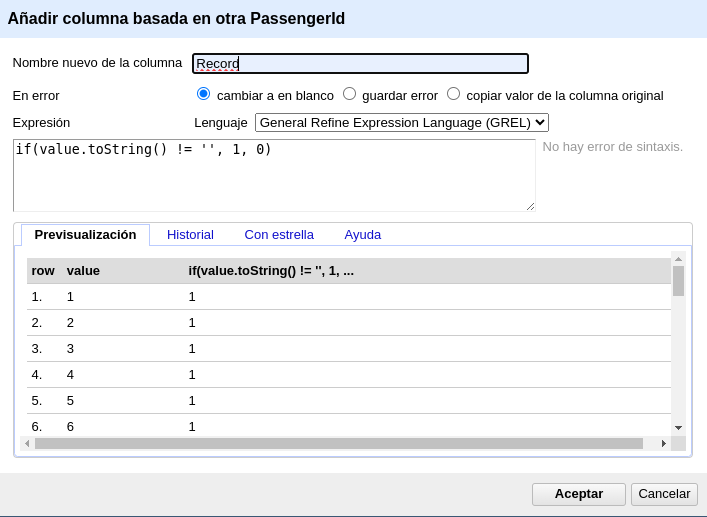
\includegraphics[width=0.6\textwidth]{img/openrefine-16.png}
                            \caption{Creando columnas a partir de otras columnas}
                        \end{figure}
                    
                    \item Reubicamos la columna \textit{Record} en la primera posición haciendo click en la columna \textit{Todo $\rightarrow$ Editar columnas $\rightarrow$ Reordenar/quitar columnas}, arrastramos la columna \textit{Record} a la primera posición y click en \textit{aceptar}.
                        \newpage
                        \begin{figure}[!h]
                            \centering
                            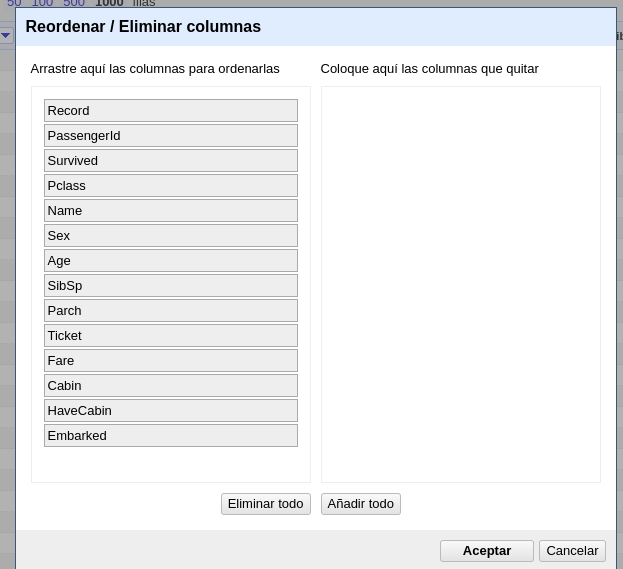
\includegraphics[width=0.6\textwidth]{img/openrefine-17.png}
                            \caption{Reordenando columnas}
                        \end{figure}
                    
                    \item Agrupamos los datos dando click en \textit{Todo $\rightarrow$  Editar celdas $\rightarrow$  Vaciar hacia abajo}.
                    \item Creamos una nueva columna a partir de \textit{Age} con el nombre \textit{AgeProm}, le agregamos el siguiente código \textit{round(sum(row.record.cells['Age'].value) / length(row.record.cells['Age'].value))} y click en \textit{Aceptar}.
                        \begin{figure}[!h]
                            \centering
                            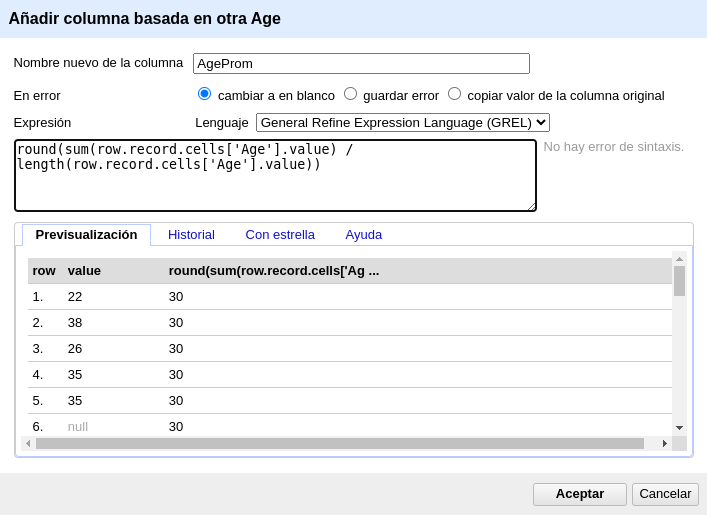
\includegraphics[width=0.6\textwidth]{img/openrefine-18.png}
                            \caption{Creando columnas a partir de otras columnas}
                        \end{figure}
                    
                    \item Para reemplazar los valores faltantes de la columna \textit{Age} por la media damos click en \textit{Age $\rightarrow$  Editar celdas $\rightarrow$  Transformar}, agregamos el código \textit{if(value.toString() == '', 30, value)} y click en \textit{Aceptar}.
                        \begin{figure}[!h]
                            \centering
                            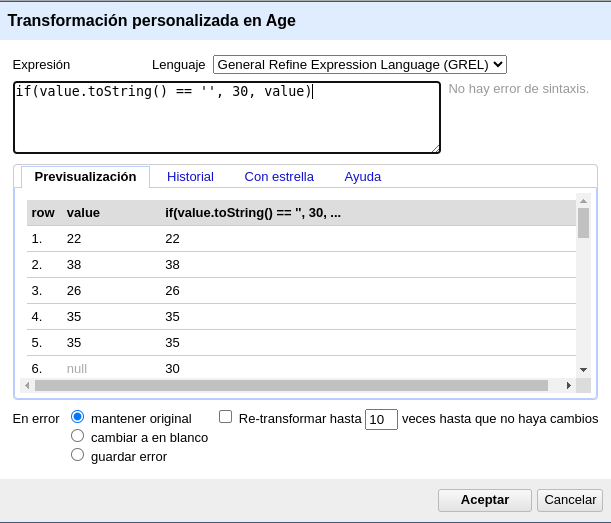
\includegraphics[width=0.6\textwidth]{img/openrefine-19.png}
                            \caption{Agregando la media de las edades en la columna Age}
                        \end{figure}
                    
                    \item Una vez preprocesada la data, ya no es necesaria la columna \textit{Record, Cabin, AgeProm}, y podemos eliminarlas, para evitar campos vacíos.
                    \item Buscamos si existen valores duplicados, en el caso de la columna \textit{PassengerId}, ordenamos la información dando click en \textit{PassengerId $\rightarrow$ Ordenar $\rightarrow$} seleccionamos \textit{números} y \textit{menores primero}, click en \textit{Aceptar}.
                        \begin{figure}[!h]
                            \centering
                            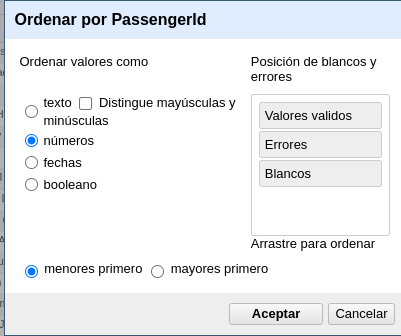
\includegraphics[width=0.5\textwidth]{img/openrefine-20.png}
                            \caption{Ordenando la columna PassengerId}
                        \end{figure}
                    
                    \item Para visualizar si existen duplicados damos click en \textit{PassengerId $\rightarrow$ Facetas $\rightarrow$ Facetas personalizadas $\rightarrow$  Faceta por duplicados}.
                        \begin{figure}[!h]
                            \centering
                            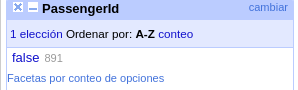
\includegraphics[width=0.4\textwidth]{img/openrefine-21.png}
                            \caption{Buscando duplicados en PassengerId}
                        \end{figure}
                    
                    \item En el caso de existir duplicados, damos cliec en \textit{PassengerId $\rightarrow$ Editar celdas $\rightarrow$ vaciar hacia abajo}, luego en \textit{PassengerId $\rightarrow$ Facetas $\rightarrow$ Facetas personalizadas $\rightarrow$ Faceta por blanco (nulo o cuerda vacía)} y en el caso de existir valores vacíos seleccionar y eliminarlos.
                    \item Para el caso de la edad creamos una columna llamada \textit{TypeAge} en base a la columna \textit{Age}, donde se considera si \textit{<18} el valor será \textit{0}, y si es \textit{>=18} el valor será \textit{1}.
                        \begin{figure}[!h]
                            \centering
                            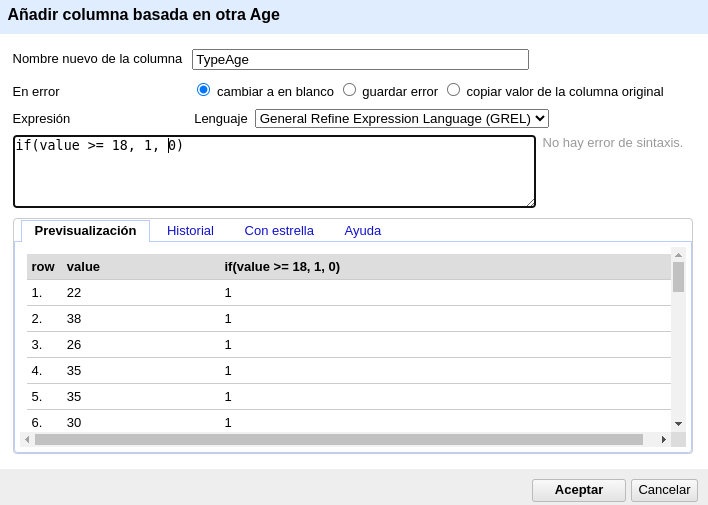
\includegraphics[width=0.6\textwidth]{img/openrefine-22.png}
                            \caption{Creando columnas a partir de otras columnas}
                        \end{figure}
                    
                    \newpage
                    \item Regresamos todos los datos a tipo cadena.
                        \begin{figure}[!h]
                            \centering
                            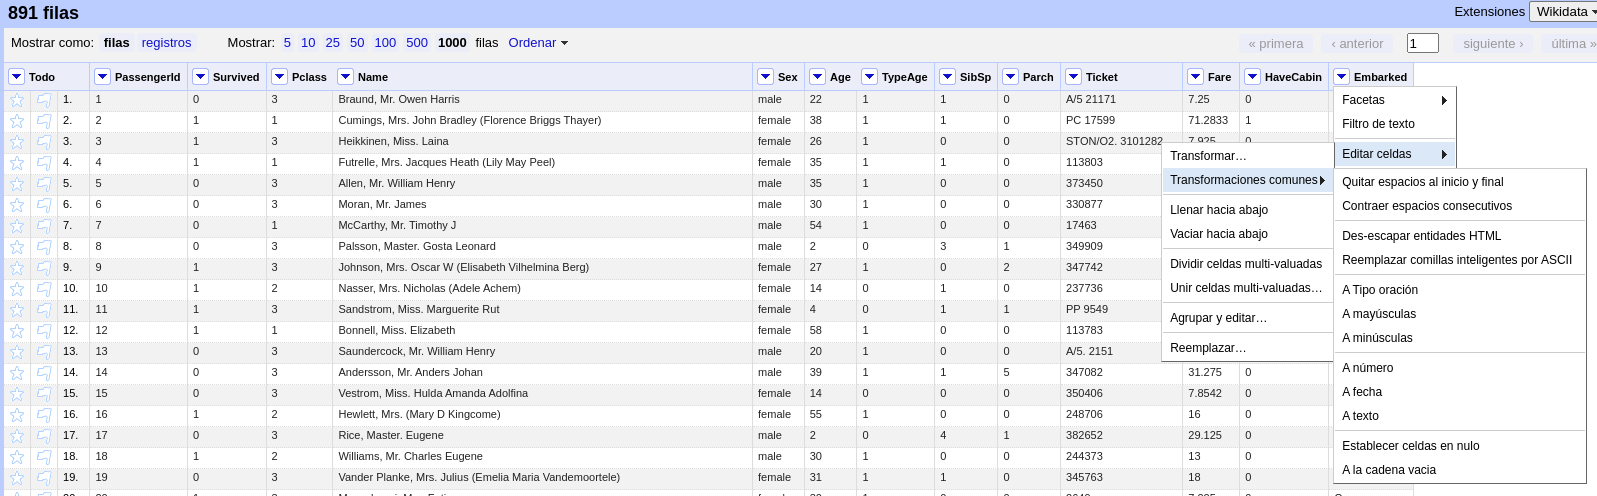
\includegraphics[width=1\textwidth]{img/openrefine-23.png}
                            \caption{Transformado a tipo de dato cadena}
                        \end{figure}
                    
                    \item Finalmente, exportamos el archivo dando click \textit{Exportar $\rightarrow$ Valor delimitado por comas} en la exquina superior derecha. Se decarga un archivo \textit{titanic-csv.csv}. Tambien podemos exportar los datos en formato excel.
                        \begin{figure}[!h]
                            \centering
                            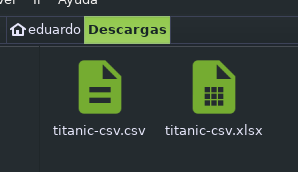
\includegraphics[width=0.3\textwidth]{img/openrefine-24.png}
                            \caption{Datos pre-procesados}
                        \end{figure}
                
                \end{itemize}
                

            \newpage
            \subsection{Weka}
                Weka es una plataforma de software libre que permite a los usuarios aplicar diversos algoritmos de aprendizaje automático y técnicas de minería de datos a sus conjuntos de datos. El nombre "Weka" proviene del nombre de un ave nativa de Nueva Zelanda y fue desarrollado por la Universidad Waikato en Nueva Zelanda.
                
                \begin{itemize}
                    \item Descargamos \href{https://waikato.github.io/weka-wiki/downloading_weka/}{\uline{Weka}} para Ubuntu. Realizamos el mismo procedimiento de instalacion de \textit{OpenRefine}, este caso, los permiso de ejecución se deben otorgar al archivo \textit{weka.sh} y para ejecutarlo con \textit{./weka.sh}.
                        \begin{figure}[!h]
                            \centering
                            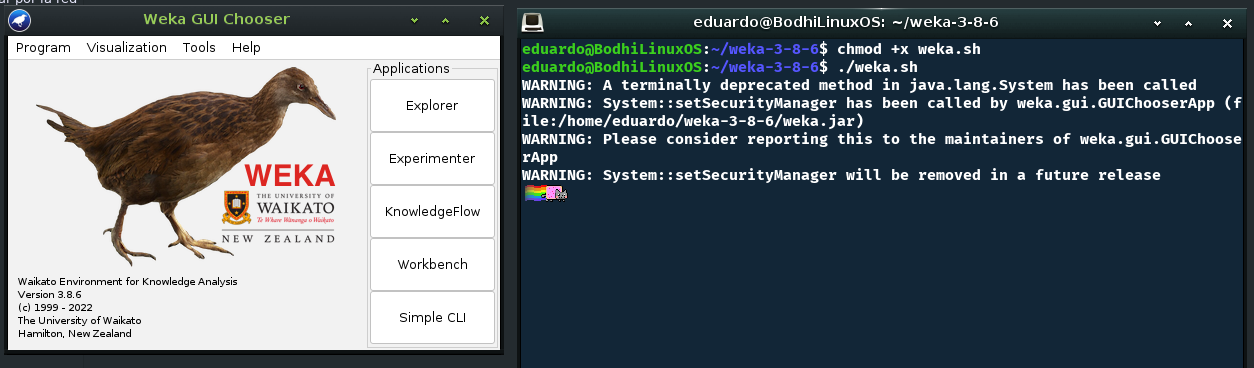
\includegraphics[width=1\textwidth]{img/weka-1.png}
                            \caption{Ejecutando Weka}
                        \end{figure}
                    
                    \item Weka ofrece las opciones posibles de interfaces de trabajo. 
                        \begin{itemize}
                            \item \textbf{Explorer:} es la opción que permite ejecutar los algoritmos de análisis y comparar resultados sobre un único conjunto de datos.
                            \item \textbf{Experimenter:} es la opción que permite definir experimentos complejos y almacenar resultados.
                            \item \textbf{Kwoledge Flow:} es la opción que permite llevar a cabo las mismas operaciones que Exprimenter pero representado como un grafo dirigido.
                            \item \textbf{Simple CLI:} es \textit{Command Line Interfaz} es una ventana de commandos java para ejecutar las clases WEKA.
                        \end{itemize}

                    \item Antes de importar el archivo \textit{.csv} preprocesado con \textit{OpenRefine} abrimos el archivo para editar caracteres que pueden ocacionar errores, en este caso reeplazamos todas las \textit{""} por un texto vacío utilizando \textit{Leafpad}, similar al \textit{Notepad++}.
                        \newpage
                        \begin{figure}[!h]
                            \centering
                            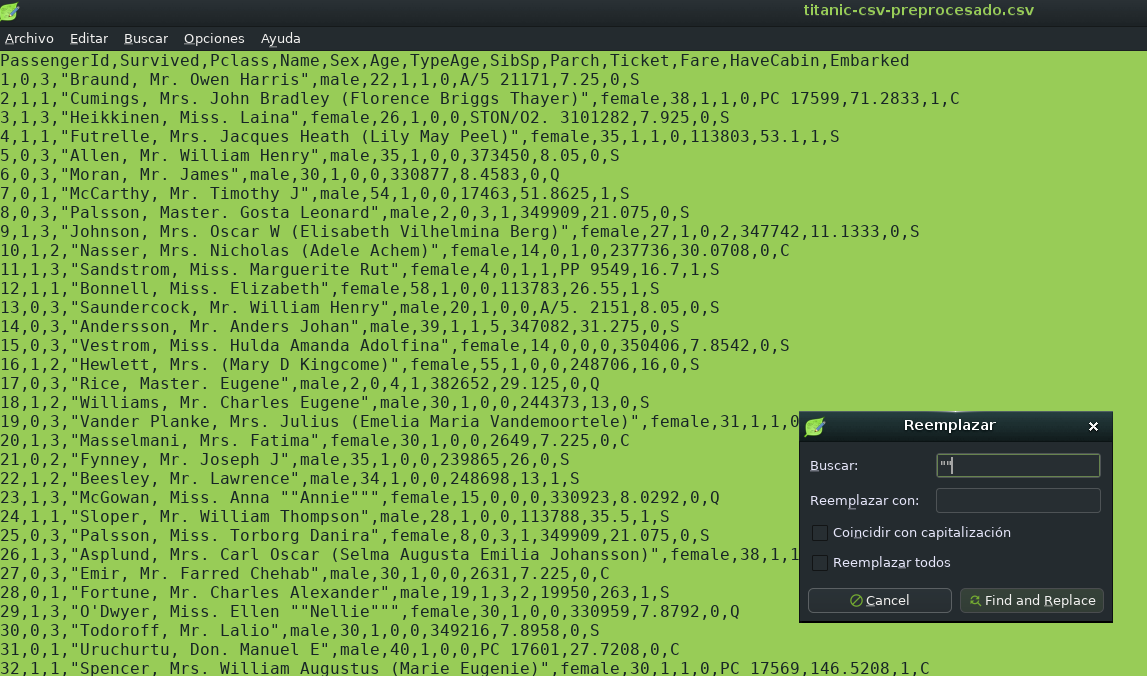
\includegraphics[width=0.7\textwidth]{img/weka-2.png}
                            \caption{Eliminando caracteres que ocacionan errores}
                        \end{figure}

                    \item Seleccionamos la opción Explorer e importamos el archivo \textit{.csv} preprocesado.
                        \begin{figure}[!h]
                            \centering
                            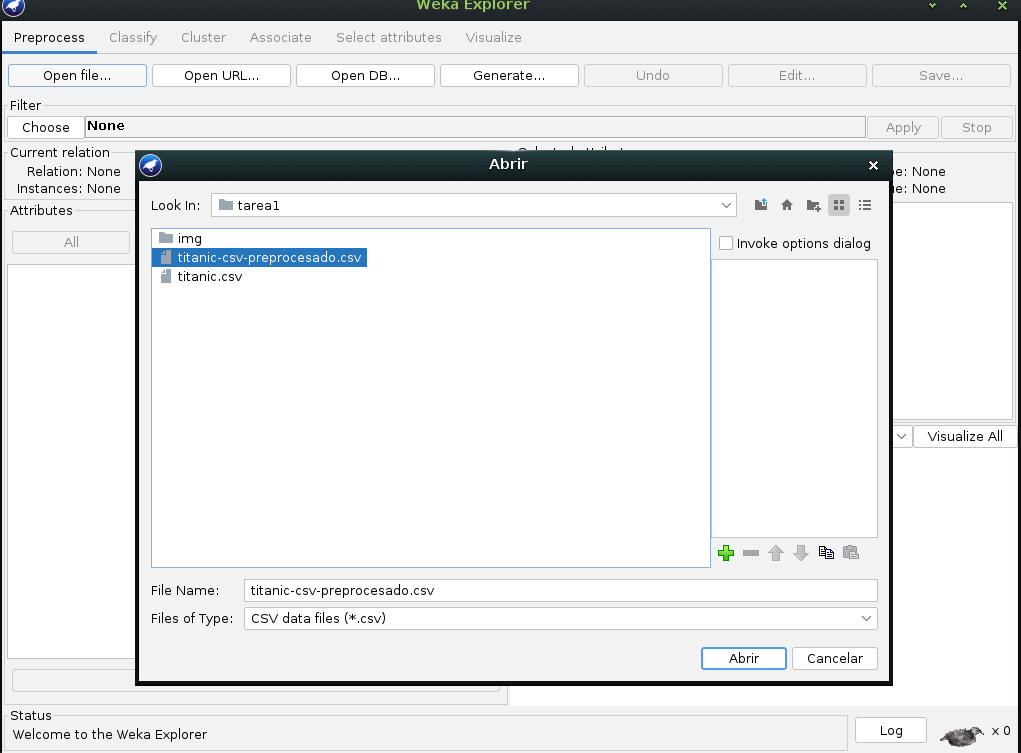
\includegraphics[width=0.6\textwidth]{img/weka-3.png}
                            \caption{Cargando una archivo .csv pre-procesado}
                        \end{figure}
                    
                    \item En esta guía se pide considerar unicamente las variables: \textit{Pclass, Age,TypeAge, Sex, Survived, Emkarked} por lo que vamos a eliminar los atributos que no se van a analizar, dando click en el botón \textit{Remove}.
                        \begin{figure}[!h]
                            \centering
                            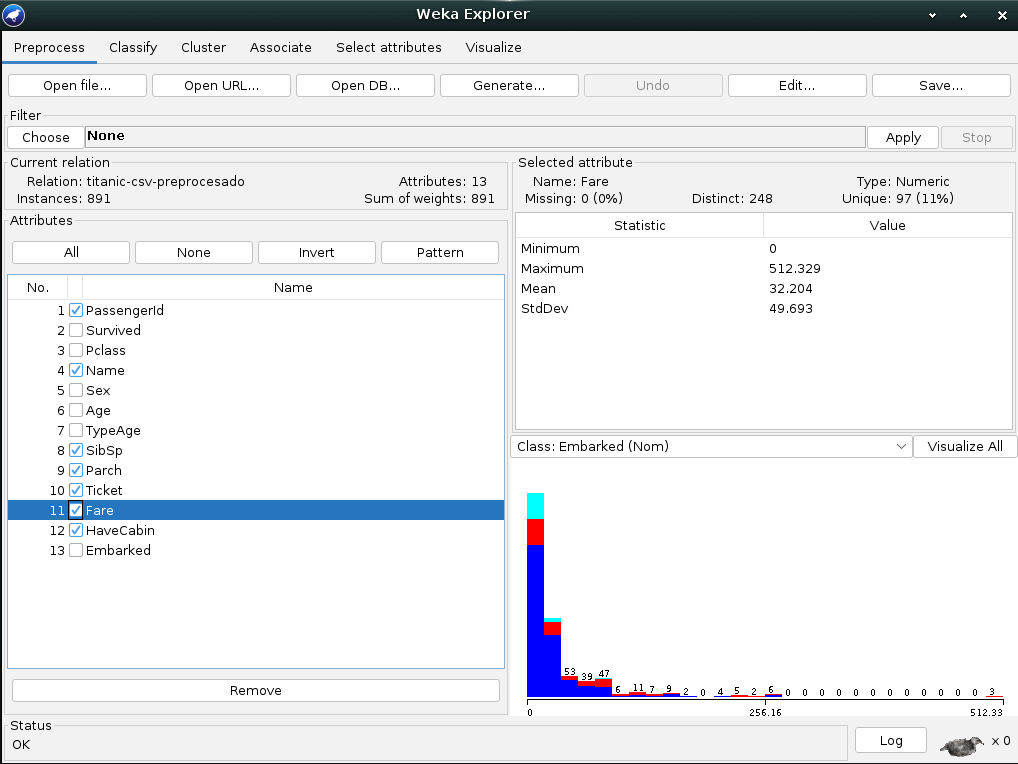
\includegraphics[width=0.6\textwidth]{img/weka-4.png}
                            \caption{Eliminando columnas inservibles}
                        \end{figure}
                    
                    \item Los atributos a analizar se componen:
                        \begin{itemize}
                            \item PClass (0 = tripulación, 1 = primera, 2 = segunda, 3 = tercera)
                            \item TypeAge (1 = adulto, 0 = niño)
                            \item Sex (1 = hombre, 0 = mujer)
                            \item Survived (1 = sí, 0 = no)
                        \end{itemize}
                        Al dar click en el botón Visualize All, nos muestra un resumen (histograma) de todas las variables:
                        \begin{figure}[!h]
                            \centering
                            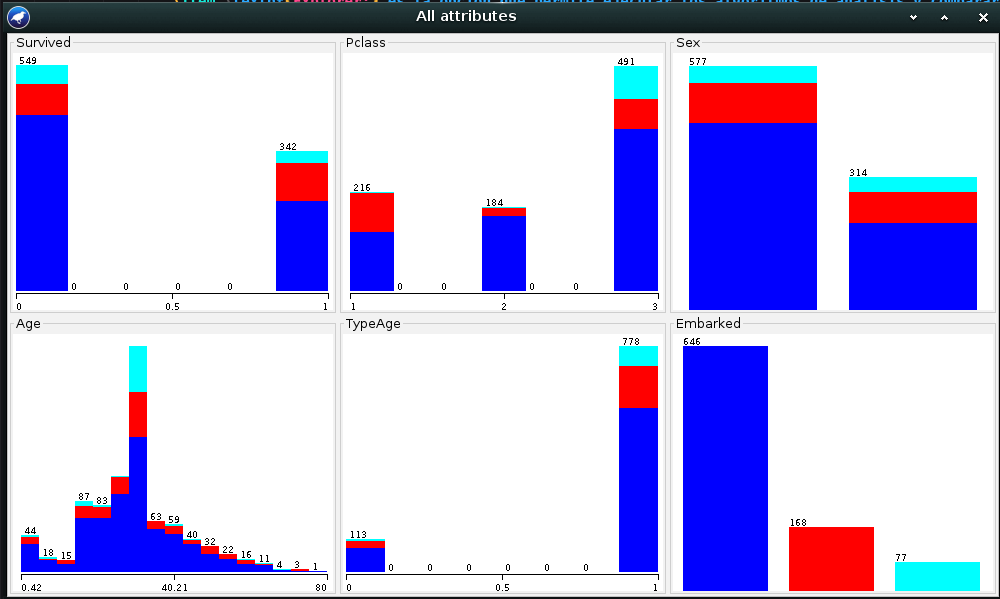
\includegraphics[width=0.6\textwidth]{img/weka-5.png}
                            \caption{Histograma de todas las variables}
                        \end{figure}

                    \item seleccionamos \textit{Filter $\rightarrow$ Choose $\rightarrow$ filters $\rightarrow$ unsupervised $\rightarrow$ attribute $\rightarrow$ NumericToNominal}, y seleccionamos las siguientes opciones:
                    \newpage
                    \begin{figure}[!h]
                        \centering
                        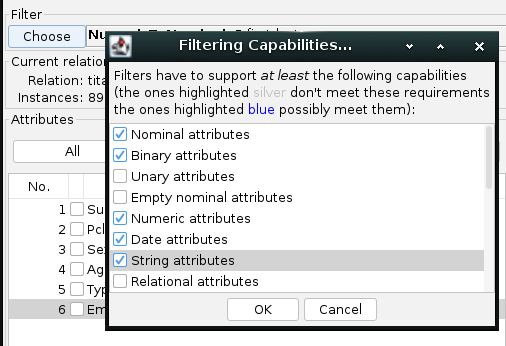
\includegraphics[width=0.5\textwidth]{img/weka-6.png}
                        \caption{Seleccionando filtros}
                    \end{figure}
                    
                    \item seleccionamos el botón \textit{Apply} de la sección de \textit{Filter}.
                        \begin{figure}[!h]
                            \centering
                            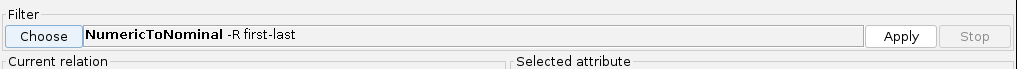
\includegraphics[width=1\textwidth]{img/weka-7.png}
                            \caption{Aplicando filtros}
                        \end{figure}
                    
                    \item Ahora podemos hacer la tarea de clasificación \textit{Classify}, Weka ofrece 4 opciones en el Test Options:
                        \begin{itemize}
                            \item \textbf{Use training set:} la muestra es usada para entrenar y probar al mismo tiempo. Los resultados obtenidos no corresponden a la realidad.
                            \item \textbf{Supplied test set:} los atributos de los datos son escritos en un nuevo archivo de formato ARFF sobre el cual se efectuará la clasificación.
                            \item \textbf{Cross-validation:} permite dividir la muestra en k partes, sobre estas se  procede a entrenar el clasificador con las k-1 partes y evaluar con la k parte actual.
                            \item \textbf{Percentage split:} indica el porcentaje de la muestra que empleara para probarel clasificador. 
                        \end{itemize}
                    
                    \item Weka ofrece 8 opciones para clasificar:
                        \begin{itemize}
                            \item \textbf{Bayes:} métodos basados en el aprendizaje de Bayes.
                            \item \textbf{Functions:} métodos matemáticos.
                            \item \textbf{Lazy:} métodos basados en el aprendizaje perezoso.
                            \item \textbf{Meta:} métodos que resultan de la combinación de diferentes métodos de aprendizaje.
                            \item \textbf{Mi:} métodos que aprenden mediante la variación de la densidad de los algoritmos.
                            \item \textbf{Misc:} métodos que aprenden como si leyeran los datos.
                            \item \textbf{Trees:} métodos que aprenden mediante árboles de decisión.
                            \item \textbf{Rules:} métodos que aprenden y estos se pueden expresar como reglas.
                        \end{itemize}

                        \begin{figure}[!h]
                            \centering
                            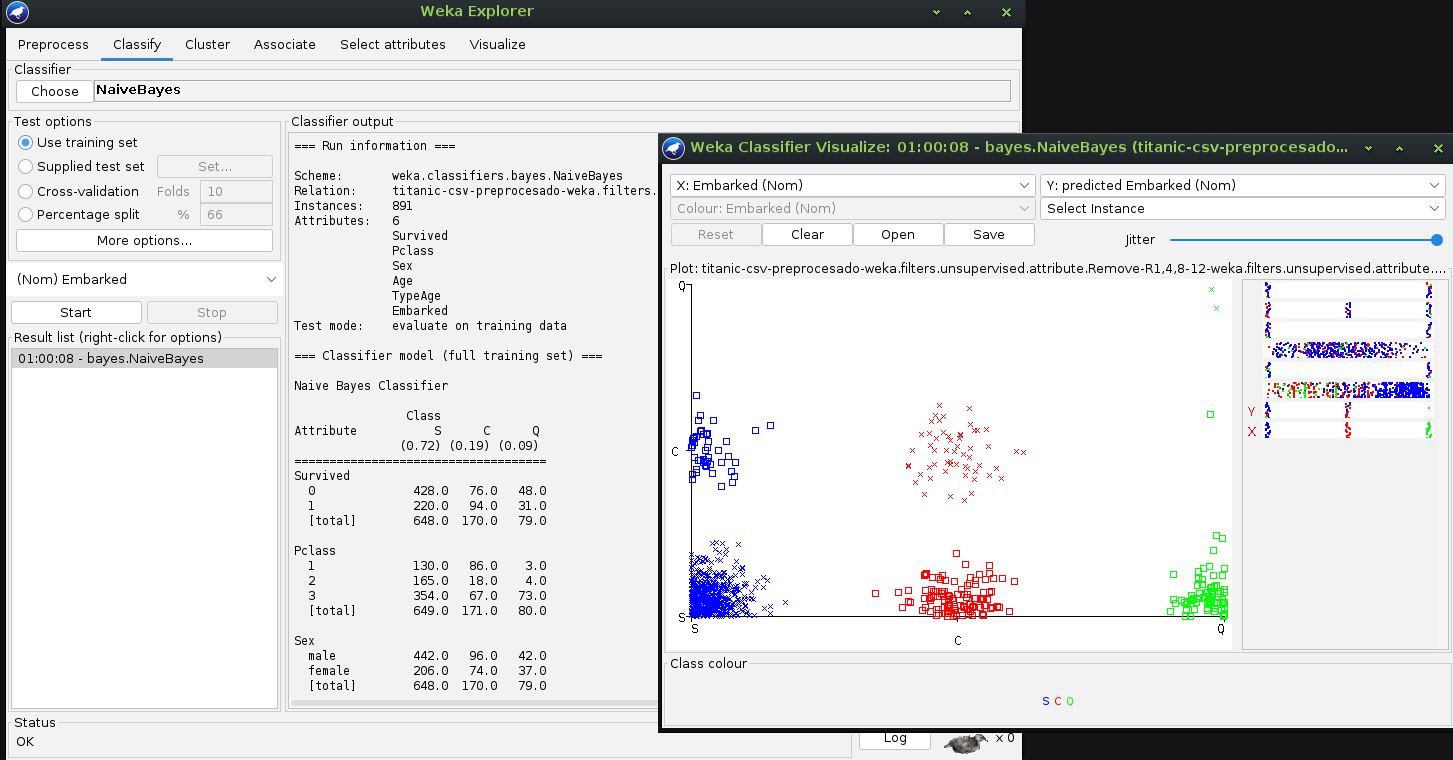
\includegraphics[width=0.9\textwidth]{img/weka-8.png}
                            \caption{Test \textit{Use training set} con opción de clasificación \textit{Bayes} - errores del clasificador}
                        \end{figure}

                        \begin{figure}[!h]
                            \centering
                            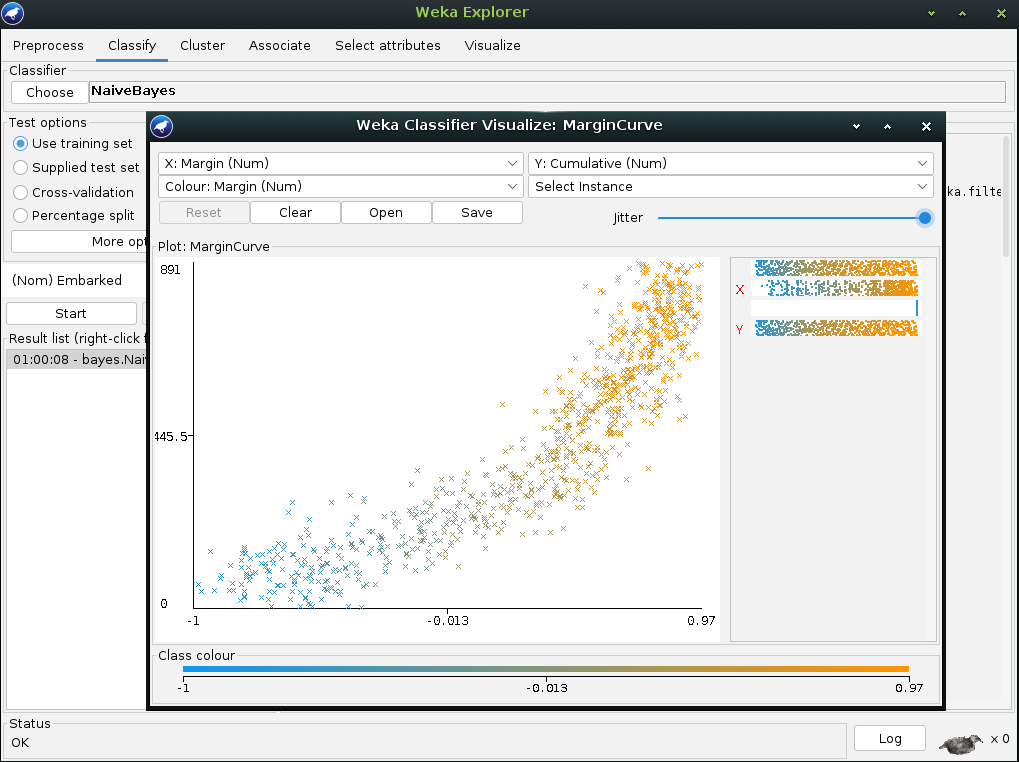
\includegraphics[width=0.8\textwidth]{img/weka-9.png}
                            \caption{Test \textit{Use training set} con opción de clasificación \textit{Bayes} - curva de margen}
                        \end{figure}

                        \newpage
                        \begin{figure}[!h]
                            \centering
                            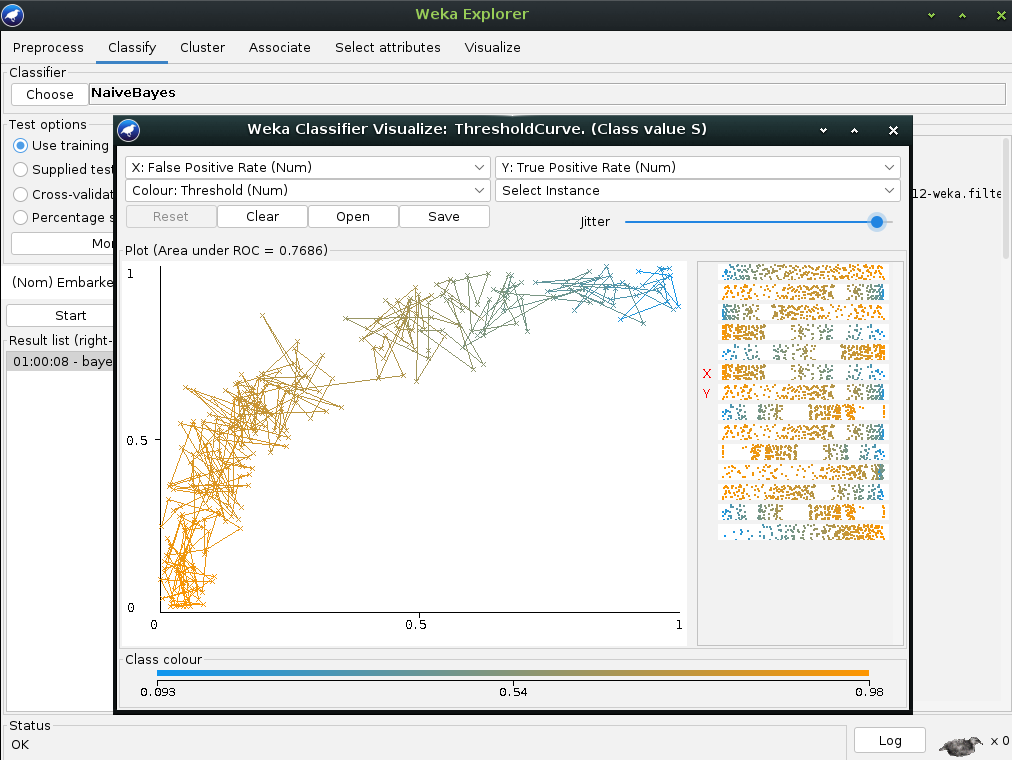
\includegraphics[width=0.8\textwidth]{img/weka-10.png}
                            \caption{Test \textit{Use training set} con opción de clasificación \textit{Bayes} - curva de umbral S}
                        \end{figure}

                        \begin{figure}[!h]
                            \centering
                            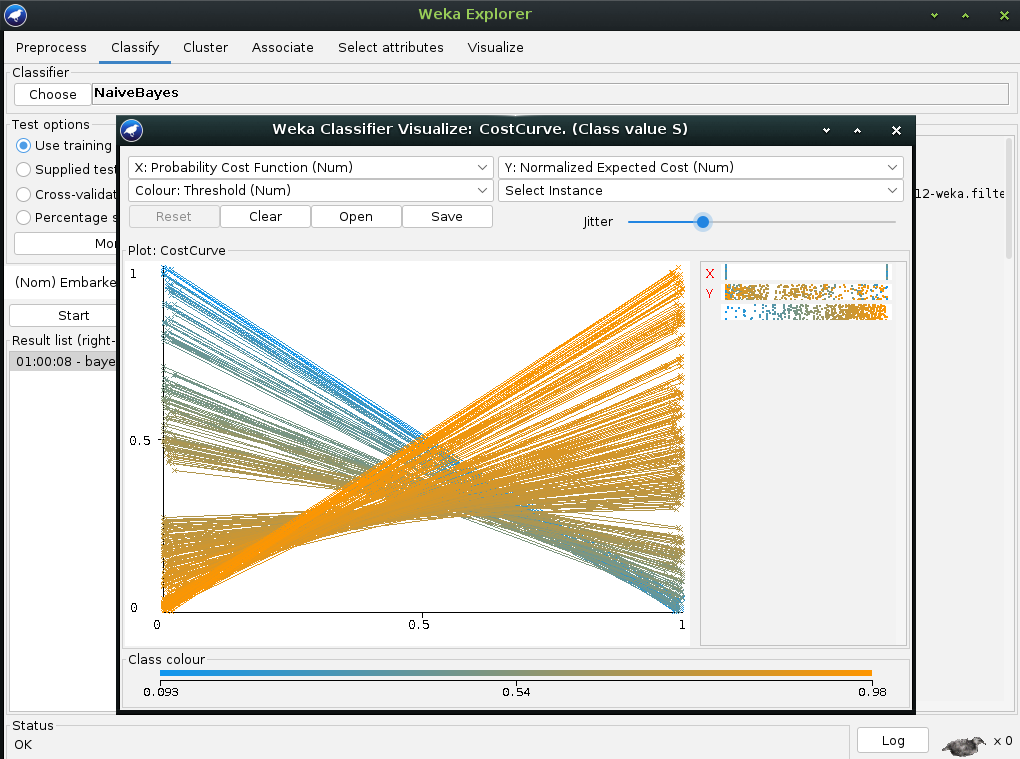
\includegraphics[width=0.8\textwidth]{img/weka-11.png}
                            \caption{Test \textit{Use training set} con opción de clasificación \textit{Bayes} - curva de costos S}
                        \end{figure}


                    \item Principales algoritmos utilizados para la clasificación:
                        \begin{itemize}
                            \item \textbf{BayesNet:}  Aprende Reyes Bayesianas.
                            \item \textbf{NaiveBayes:} Clasificador discriminador de Bayes.
                            \item \textbf{Id3:} Arboles de decisión usando el divide y vencerás.
                            \item \textbf{J48:} Arboles de decisión usando el C4.5.
                            \item \textbf{RandomForest:} Construye un bosque aleatorio.
                            \item \textbf{JRip:} Construye reglas con el algoritmo RIPPER.
                            \item \textbf{M5Rules:} Construye reglas M5 desde árboles.
                            \item \textbf{LinearRegression:} Utiliza la regresión lineal.
                            \item \textbf{MultilayerPerceptron:} Usa red neuronal de Retroprogramación.
                            \item \textbf{RBFNetwork:} Usa Red de función en Radio base.
                            \item \textbf{SMO:} basado en vectores de soporte.
                            \item \textbf{Ibk:} Usa k vecinos más cercanos.
                            \item \textbf{LWL:} Aprendizaje basados en Pesos Locales.
                            \item Entre muchos otros.
                        \end{itemize}
                    
                    \item Weka ofrece cuatro opciones en Cluster mode:
                        \begin{itemize}
                            \item \textbf{Use training set:} la muestra es usada para entrenar y probar al mismo tiempo. Los resultados obtenidos no corresponden a la realidad.
                            \item \textbf{Supplied test set:}  los atributos de los datos son escritos en un nuevo archivo de formato ARFF sobre el cual se efectuará la clasificación.
                            \item \textbf{Percentage split:}  indica el porcentaje de la muestra que empleara para probar el clasificador. 
                            \item \textbf{Classes to cluster evaluation:} permite escoger el atributo a agrupar.
                        \end{itemize}

                        \newpage
                        \begin{figure}[!h]
                            \centering
                            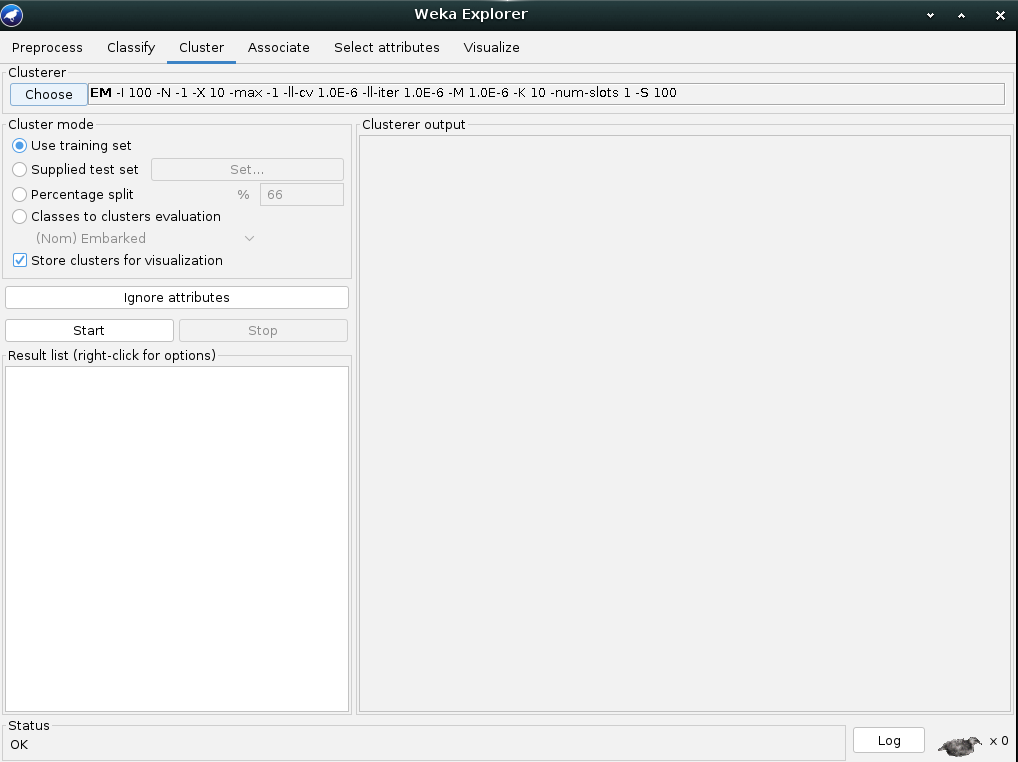
\includegraphics[width=0.8\textwidth]{img/weka-12.png}
                            \caption{Opción de Cluster}
                        \end{figure}

                    \item Weka ofrece los algoritmos para agrupar datos:
                        \begin{itemize}
                            \item \textbf{Canopy:} Utiliza el algoritmo Canopy.
                            \item \textbf{CobWeb:} Utiliza el algoritmo CoWeb.
                            \item \textbf{EM:} Utiliza el algoritmo EM.
                            \item \textbf{FarthestFirst:} Utiliza el algoritmo FarthestFirst.
                            \item \textbf{FilteredClusterer:} agrupa los datos arbitrariamente y luego son pasados por un filtro arbitrario.
                            \item \textbf{HierarchicalClusterer:} agrupa los datos jerarquicamente y luego son pasados por un filtro arbitrario.
                            \item \textbf{MakeDensityBasedClusterer:}  los datos son envueltos en clases y devuelven su distribución y densidad.
                            \item \textbf{OPTICS:} utiliza el algoritmo OPTICS.
                            \item \textbf{SimpleKMeans:} utiliza el algoritmo de k-medias.
                        \end{itemize}

                        \newpage
                        \begin{figure}[!h]
                            \centering
                            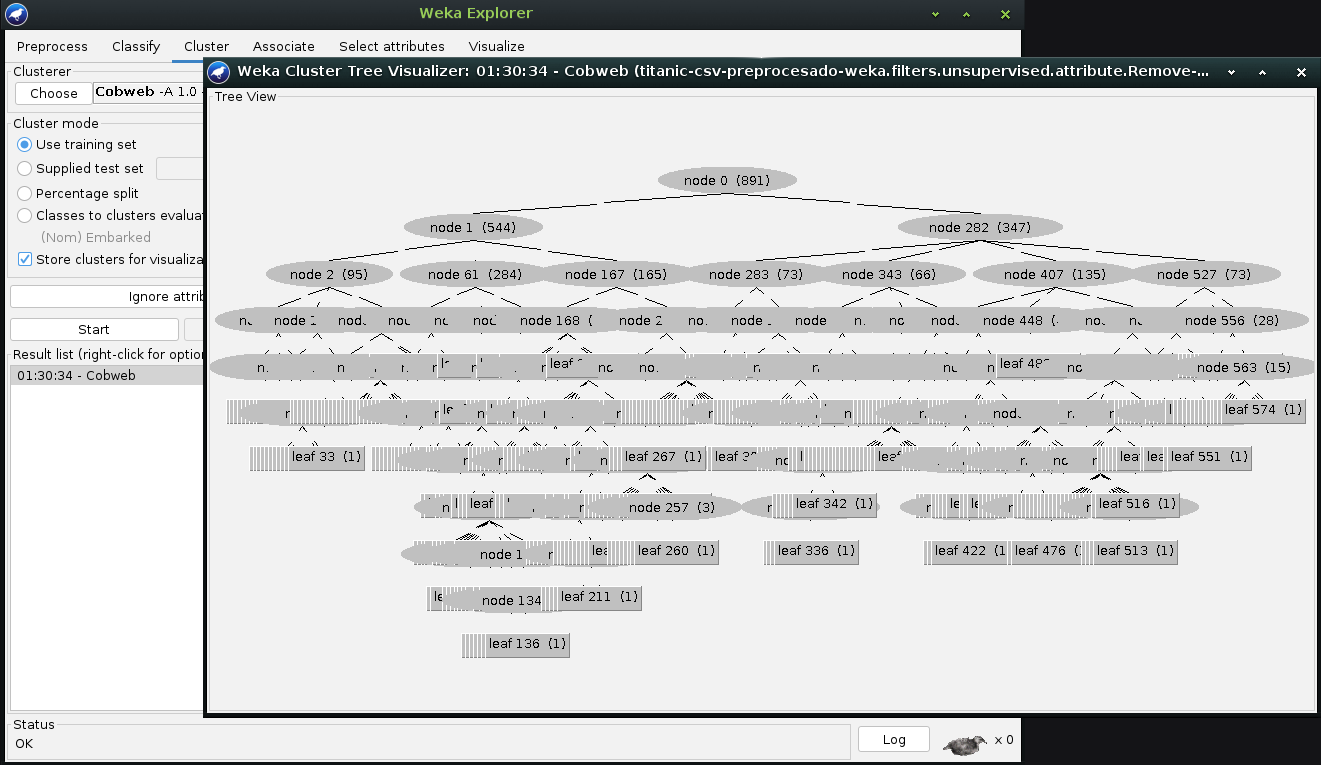
\includegraphics[width=0.8\textwidth]{img/weka-13.png}
                            \caption{Cluster - \textit{CobWeb} - \textit{Use training set} - visualizar árbol}
                        \end{figure}

                        \begin{figure}[!h]
                            \centering
                            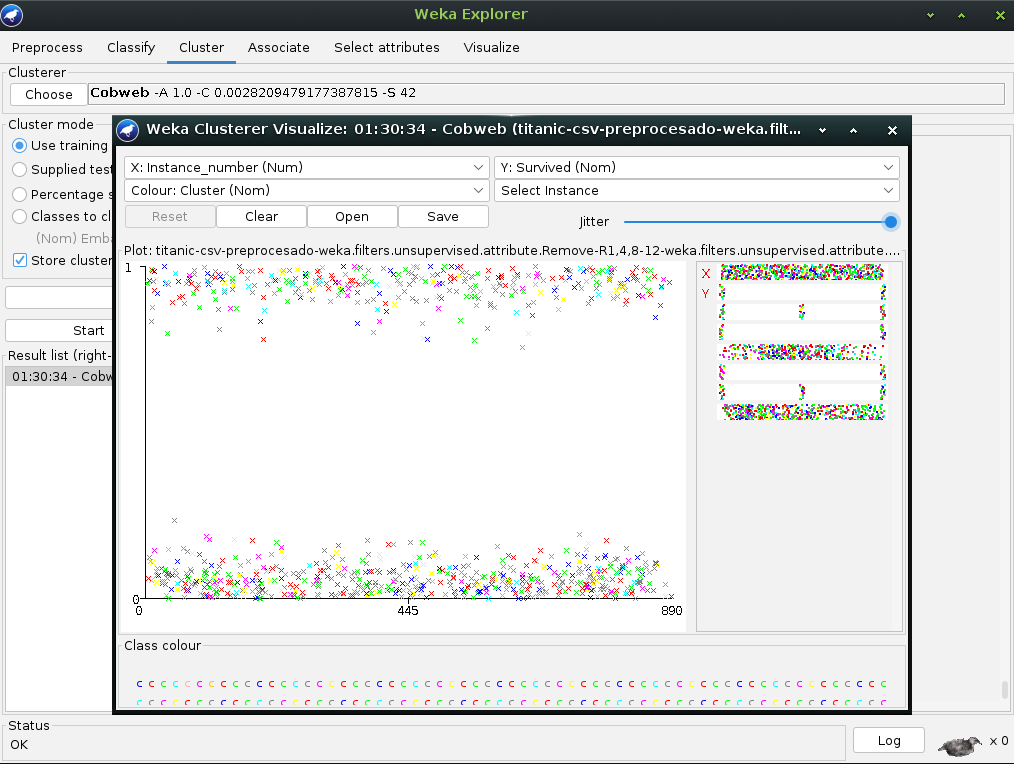
\includegraphics[width=0.8\textwidth]{img/weka-14.png}
                            \caption{Cluster - \textit{CobWeb} - \textit{Use training set} - visualizar asignaciones de clúster}
                        \end{figure}

                    \item Para ejecutar los métodos en Weka de reglas de asociación, seleccionamos la ventana de \textit{associate}, Weka ofrece los algoritmos para asociar datos:
                        \begin{itemize}
                            \item \textbf{Apriori:} Utiliza el algoritmo Apriori.
                            \item \textbf{FilteredAssociator:}  utiliza el algoritmo que asocia los datos arbitrariamente y también los filtra arbitrariamente.
                            \item \textbf{FPGrowth:} El algoritmo de crecimiento FP representa la base de datos en forma de árbol llamado árbol de patrones frecuentes o árbol FP.
                        \end{itemize}
                        
                        \begin{figure}[!h]
                            \centering
                            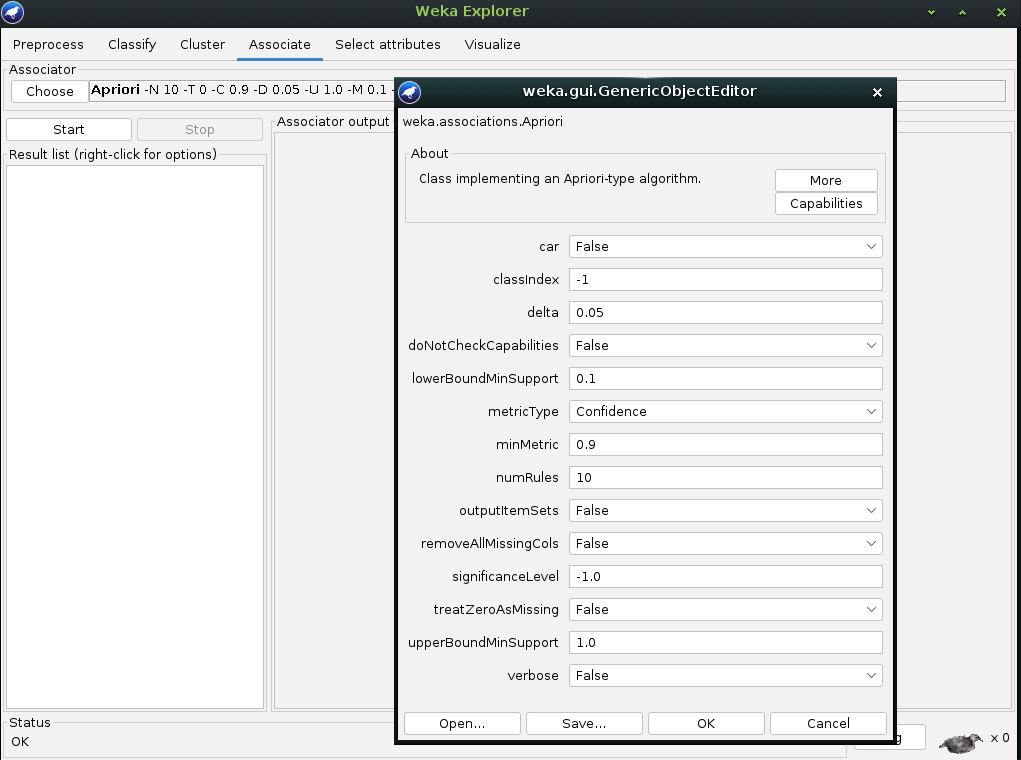
\includegraphics[width=0.8\textwidth]{img/weka-15.png}
                            \caption{Técnica de minería de datos - Apriori por defecto}
                        \end{figure}

                        \begin{figure}[!h]
                            \centering
                            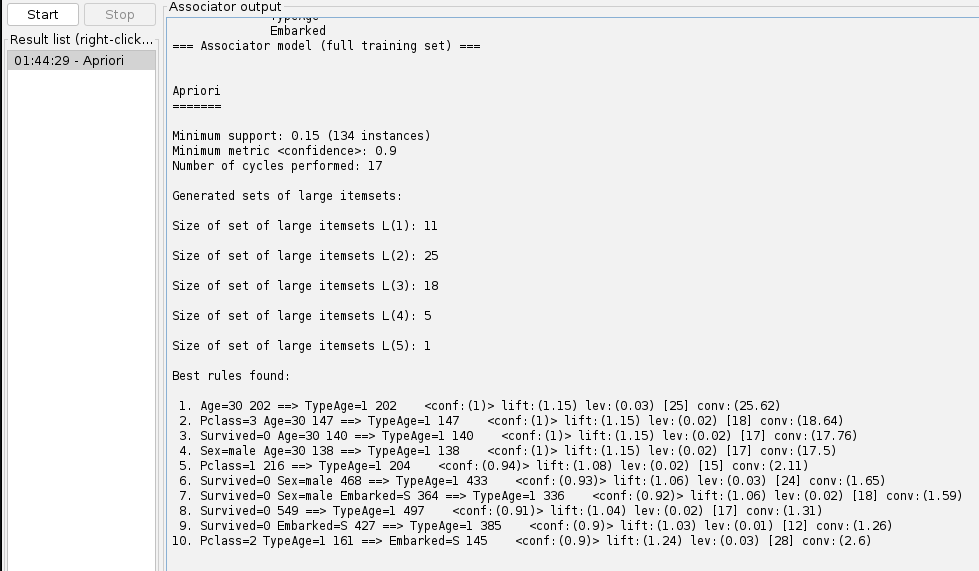
\includegraphics[width=0.8\textwidth]{img/weka-16.png}
                            \caption{Técnica de minería de datos - Apriori por defecto}
                        \end{figure}

                        En cada regla, tenemos la cobertura de la parte izquierda y de la regla, así como la confianza de la regla. Por ejemplo, la regla 1 indica que, como se supone todas las personas de la clase 1 son adultas. La regla 4 nos indica lo mismo que regla 1, pero teniendo en cuenta a los varones. Parecidas conclusiones se pueden observar de la regla 2,5 y 10. La regla 6 nos indica que los varones que murieron fueron en su mayoría adultos 93\%. La regla 8 nos indica que la mayoría que murieron eran adultos 91\%. Y finalmente, la regla 7 nos indica que la mayoría de muertos fueron hombres 91\%.

                        \begin{figure}[!h]
                            \centering
                            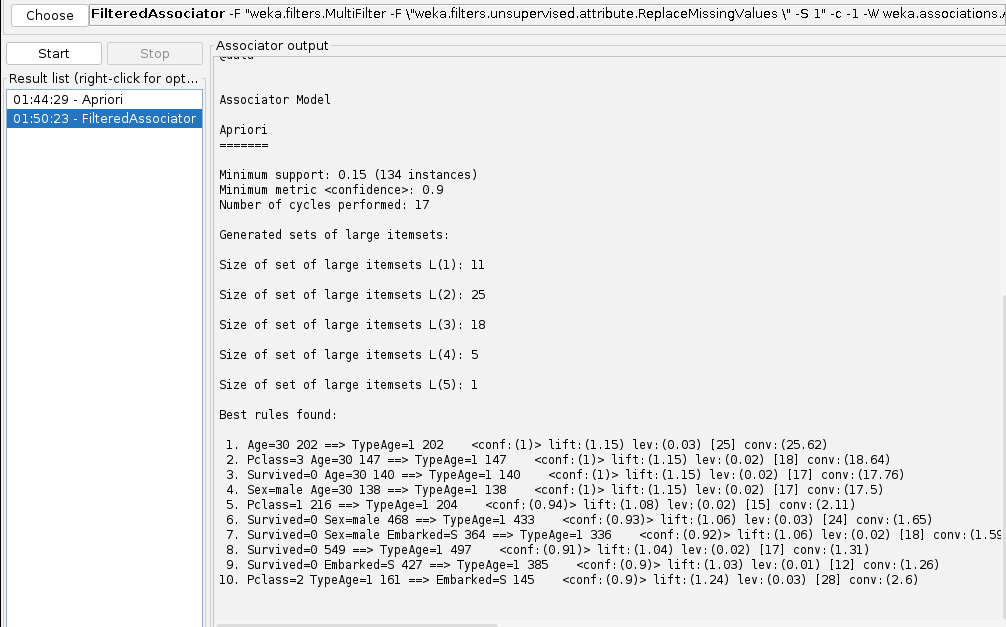
\includegraphics[width=0.8\textwidth]{img/weka-17.png}
                            \caption{Técnica de minería de datos - FilteredAssociator}
                        \end{figure}

                    \newpage
                    \item Visualización:
                        \begin{figure}[!h]
                            \centering
                            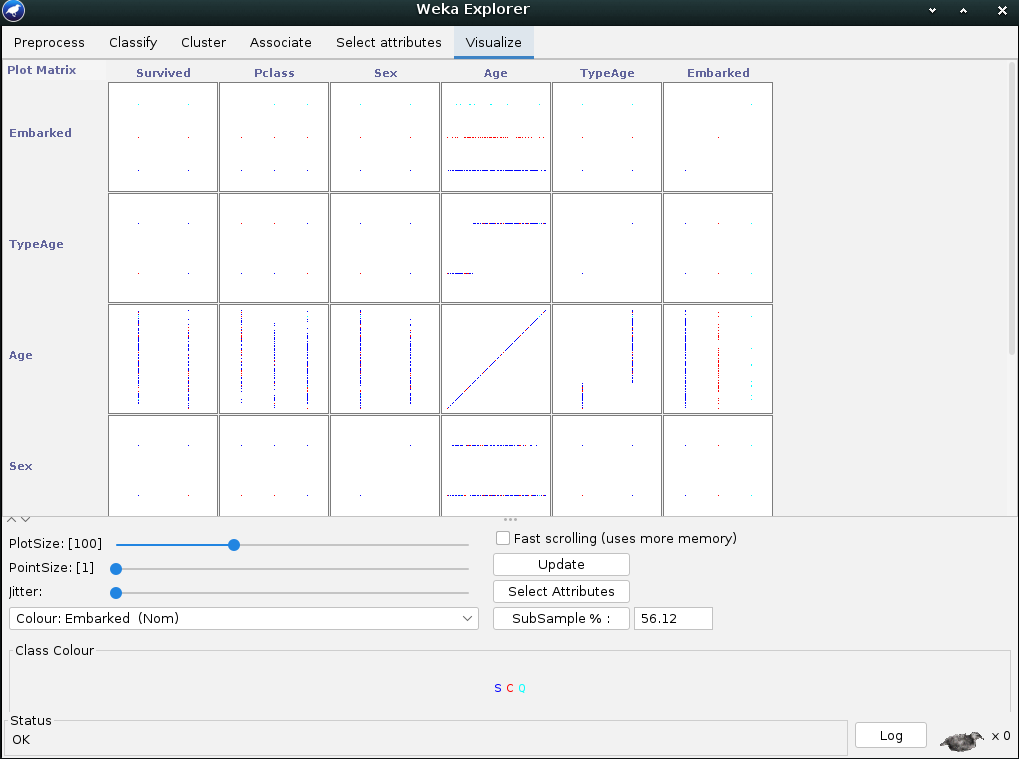
\includegraphics[width=0.7\textwidth]{img/weka-18.png}
                            \caption{Visualización}
                        \end{figure}

                        \begin{figure}[!h]
                            \centering
                            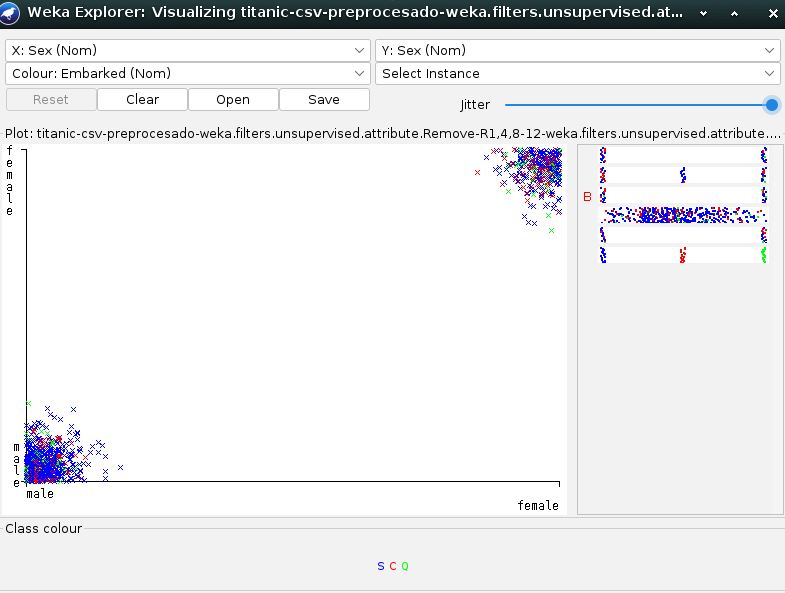
\includegraphics[width=0.7\textwidth]{img/weka-19.png}
                            \caption{Visualización}
                        \end{figure}

                \end{itemize}


    % 4.Errores y correcciones: ...................................................
    \newpage
    \section{Errores y correcciones realizadas a la data}
        Durante el proceso de limpieza y preprocesamiento de la data del archivo titanic.csv, se identificaron varios errores típicos:

        \begin{itemize}
            \item Primero, se renombraron columnas con nombres genéricos, como Column, a nombres más descriptivos, como Vacia. 
            \item Se transformaron columnas con valores numéricos (Survived, PClass, Sibsp, Parch, Age, Fare) de formato de cadena a sus respectivos tipos numéricos. 
            \item Se identificaron valores nulos en las columnas Age, Cabin y Embarked.
            \item Para Embarked, los valores faltantes se reemplazaron con "S", indicando Southampton.
            \item En el caso de Cabin, se creó una columna adicional llamada HaveCabin para marcar con 1 si la cabina existe y con 0 si no existe. 
            \item Los valores nulos en Age se reemplazaron con la media de la columna.
            \item Se eliminaron las columnas innecesarias, como Vacia, Record, Cabin, y AgeProm, una vez que ya no eran útiles. 
            \item Para manejar posibles duplicados en PassengerId, se identificaron y eliminaron registros duplicados. 
            \item Adicionalmente, se creó la columna TypeAge para clasificar edades en menores de 18 (0) y mayores o iguales a 18 (1). 
            \item Finalmente, todos los datos se regresaron a tipo cadena para mantener la consistencia en el formato.
        \end{itemize}

    % 5.Resultados: ...................................................
    \newpage
    \section{Resultados del análisis de la data}
        Usando Weka para analizar los datos preprocesados del Titanic, se pueden obtener varios resultados:

        \begin{itemize}
            \item Los algoritmos de clasificación, como NaiveBayes, J48 (árbol de decisión), y RandomForest, permitirán predecir la probabilidad de supervivencia de los pasajeros basándose en atributos como Pclass, TypeAge, Sex, y Embarked. Por ejemplo, se puede identificar que los pasajeros de primera clase tenían una mayor probabilidad de supervivencia. 
            \item Utilizando reglas de asociación como el algoritmo Apriori, se pueden descubrir patrones significativos, como que la mayoría de los adultos varones no sobrevivieron, mientras que muchas mujeres y niños sí lo hicieron. Además, con algoritmos de agrupamiento como k-means, se pueden segmentar los pasajeros en grupos con características similares, lo cual podría revelar insights sobre la distribución y comportamiento de diferentes grupos en el barco. 
            \item La visualización de estos análisis a través de histogramas y gráficos facilitará la interpretación y comunicación de los resultados, permitiendo una comprensión más clara de los factores que influyeron en la supervivencia durante el hundimiento del Titanic.
        \end{itemize}

    % 6.Conclusiones: ...................................................
    \newpage
    \section{Conclusiones y recomendaciones}
        \subsection{Conclusiones}
            \begin{enumerate}
                \item Aprendimos a utilizar Kaggle para acceder a conjuntos de datos reales. 
                \item Simplificamos la limpieza y preparación de datos utilizando OpenRefine, mejorando nuestra habilidad en la manipulación de datos.
                \item Repasamos de manera muy superficial sobre los diferentes algoritmos de aprendizaje automático con Weka, como clasificación y agrupamiento.
                \item Analizamos el dataset del Titanic para obtener insights prácticos sobre la supervivencia en contextos históricos.
                \item Desarrollamos habilidades analíticas al aplicar técnicas de análisis de datos en un problema reales de ciencia de datos.
                \item Integramos Kaggle, OpenRefine y Weka para mejorar nuestra capacidad en la toma de decisiones basadas en datos.
            \end{enumerate}

        \subsection{Recomendaciones}
            \begin{enumerate}
                \item Proporcionar una explicación más detallada sobre el uso de la aplicación Weka, enfocándose en hacer la herramienta accesible para estudiantes con menos experiencia técnica.
                \item Explorar con mayor profundidad conceptos avanzados en aprendizaje automático y sus diversos algoritmos.
            \end{enumerate}
    % 7.Bibliografía: ...................................................
    \newpage
    \section{Bibliografía}
        \begin{itemize}
            \item Invitado. (2016, 6 julio). Open Refine – qué es + tutorial. Escuela de Datos. \\https://es.schoolofdata.org/2014/06/30/openrefine/index.html
            \item Isaiaranda. (2021, 16 diciembre). ¿QUE ES WEKA? - Isaiaranda - Medium. Medium. \\https://medium.com/@isaiaranda15/que-es-weka-926c05050d44
            \item Guía practica proporcionada por la docente.
        \end{itemize}

\end{document}